\section{Technical standards}
\label{sect:standards}
In this section we define explicitly the technical data exchange format for the
logical structures defined in the previous subsections.

%%%%%%%%%%%%%%%%%%%%%%%%%%%%%%%%%%%%%%%%%%%%%%%%%%%%%%%%%%%%%%%%%%%%%%%%%%%%%%%
\subsection{Object model}
The validation report structure consists of records that are either of
type validation, or aggregation. The former are schematically represented as
follows
\begin{align*}
\textsf{validation}&:=\langle
  \textsf{id}
, \textsf{type}=\code{"validation"}
, \textsf{event}
, \textsf{rule}
,\textsf{data}
,\textsf{value}\rangle\\
\textsf{event} &:= \langle
  \textsf{time}
, \textsf{actor}
, agent
, trigger\rangle\\
\textsf{rule} &:=\langle
  \textsf{language}
, \textsf{expression}
, \textsf{severity}
, status
, decription\rangle\\
\textsf{data} &:=\langle
  \textsf{source}
, \textsf{target}
, description\rangle,
\end{align*}
where `id' is a unique identifier, `type' has a fixed value that labels the
object type and `value' is a validation result ($0$, $1$ or $\na{}$). In the
above scheme, the fields in $italics$ are optional. 

Objects of type type `aggregation' are schematically described as
\begin{align*}
\textsf{aggregation} &:=\langle
  \textsf{id}
, \textsf{type}=\code{"aggregation"}
, \textsf{event}
, \textsf{aggregate}
, \textsf{data}
,\textsf{value}\rangle\\
\textsf{event} &:= \langle
  \textsf{time}
, \textsf{actor}\rangle\\
\textsf{aggregate} &:=\langle
  \textsf{language}
, \textsf{expression}
, description\rangle\\
\textsf{data} &:=\langle
  \textsf{source}
, \textsf{target}
, description\rangle,
\end{align*}
where `value' is the aggregate value, represented as a string.

The above description serves as a quick reference data structure, independent
of the implementation language. It encompasses
Definitions~\ref{def:validationresult}, \ref{def:confrontation} and
\ref{def:aggregation}, with components derived from the logical descriptions in
\S\ref{sect:basicreportstructure}.

%%%%%%%%%%%%%%%%%%%%%%%%%%%%%%%%%%%%%%%%%%%%%%%%%%%%%%%%%%%%%%%%%%%%%%%%%%%%%%%
\subsection{Implementation}

Below we propose a technical format for exchanging data
validation reports. There are several common standards allowing for
implementation of structured data exchange, including textual formats such as
XML \citep{xml}, YAML \citep{yaml}, JSON \citep{ecma2013json} and popular binary
formats such as protobuf \citep{protobuf}. In principle, any of these formats
can be used to serialize the validation and aggregation data structures that
were in the previous subsection. Here, we use the JSON format because of
simplicity, wide support in many languages, and the availability
of a schema definition language \citep{galiegue2013json}. Moreover, JSON
strings parse straight into javascript objects, facilitating further processing
and visualisation, for example in the popular \texttt{d3.js} framework
\citep{bostock2011data}. This implementation can be used as a reference and it
is left to the user to implement the concepts in another language if so
desired.


Although it is a textual format, the JSON standard does not impose restrictions
on the encoding used. It is left explicitly to standards built upon JSON to
define an encoding \citep[pp ii]{ecma2013json}. In this standard we follow the
currently most widely applied standard (see Figure~\ref{fig:encoding}) with the
following demand.

\begin{center}
\captionof{table}{File encoding used for validation reports}
\label{tab:encoding}
\begin{tabular}{|p{0.97\textwidth}|}
\hline
Validation reports  are encoded in \code{UTF-8}.\\
\hline
\end{tabular}
\end{center}

\begin{figure}[t]
\centering
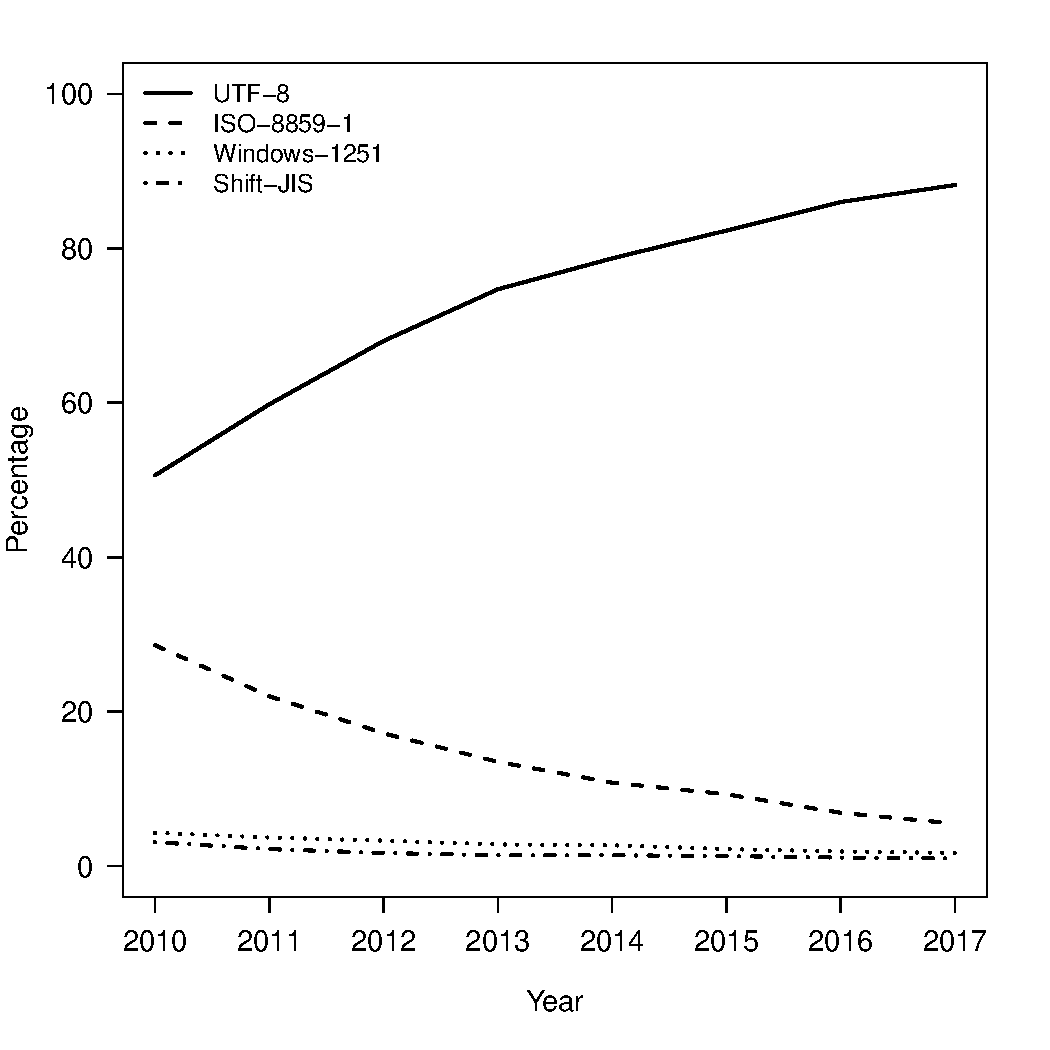
\includegraphics[width=0.7\textwidth]{fig/encoding_use.pdf}
\caption{Percentages of encoding standards used on the web \citep{w3techs2017}.}
\label{fig:encoding}
\end{figure}

The different data types within a file are to be formatted according to
commonly used standards where possible. In particular, data in validation
reports are encoded as stated in Table~\ref{tab:dataformat}.
\begin{center}
\captionof{table}{Format of data types in validation reports.}
\begin{tabular}{|lp{0.92\textwidth}|}
\hline
1&Numbers are encoded in a valid decimal ISO/IEC/IEEE 60559:2011 (IEEE 754) format
\citep{ieee:2008}. \\
2&Date-time data shall be denoted in basic ISO 8601 format \code{YYYYMMDDThhmmss}$\pm$\code{hhmm} \citep{iso2004data}. \\
\hline
\end{tabular}
\label{tab:dataformat}
\end{center}






The JSON scheme defining is shown in Listing~\ref{lst:valrep1}. The full code
can also be found at github:
\begin{center}
\href{https://github.com/data-cleaning/ValidatReport}{https://github.com/data-cleaning/ValidatReport}
\end{center}

\newpage
\lstinputlisting[frame=single
  , linewidth=1.15\textwidth
  , caption=JSON schema for a validation report.
  , label=lst:valrep1]{../json/validation_report.json}

\label{lst:valrep3}
%
%
\newpage




